\documentclass[11pt]{article}

\usepackage[margin=1in]{geometry}
\usepackage{microtype}
\usepackage{booktabs}
\usepackage{amsmath}
\usepackage{graphicx}
\usepackage{xcolor}
\usepackage{listings}
\usepackage[hidelinks]{hyperref}
\usepackage{tikz}
\usetikzlibrary{arrows.meta,positioning,shapes.geometric}
\emergencystretch=2em
\sloppy

\lstset{
  basicstyle=\ttfamily\small,
  breaklines=true,
  frame=single,
  backgroundcolor=\color{black!3},
  columns=fullflexible
}

\title{\textbf{Consumable API Token Budgets in an Unmodified Two-Level Resource Broker}}

\author{
  David Palaitis\\
  \textit{Medios Lab}\\
  \texttt{https://github.com/medios-lab/medios-tokens}
}

\date{November 2026 \quad (\textit{Research Preview Technical Note})}

\begin{document}
\maketitle

\begin{abstract}
Cluster schedulers allocate reusable hardware (CPUs, memory, GPUs), while LLM API gateways enforce spend limits on the HTTP data plane after tasks have already launched. When multiple agents share a finite API budget, this split lets schedulers launch partial workflows that later fail with HTTP~429 errors.

This note describes \texttt{medios-tokens} (research preview), an out-of-process HTTP Resource Provider for Medios that advertises a consumable API token budget (\texttt{reserve} $\rightarrow$ \texttt{spend} $\rightarrow$ \texttt{settle} $\rightarrow$ \texttt{refill}) inside standard resource offers without modifying the Medios broker. We document two task-level settlement protocols---executor finish hooks (\texttt{TaskInfo.finish}) and per-task OpenRouter keys revoked on terminal task state---and report three live experiments on unmodified Medios binaries. In a six-workflow multi-agent contention test over a 100-unit pool, exposing remaining budget in resource offers allowed a budget-aware scheduler to complete $6/6$ workflows ($4/4$ high-value, $0$ wasted units) where a naive FIFO queue completed $2/6$ ($0/4$ high-value, $44.0$ units spent on stranded chains).
\end{abstract}

\section{Introduction}
\label{sec:intro}

In a two-level resource broker such as Mesos~\cite{hindman2011mesos} or Medios, the controller manages offers, allocations, and task state while external frameworks implement scheduling policy. The broker does not interpret resource semantics: it tracks typed scalar values and forwards them in offers.

We evaluate two external resource extensions against an unmodified Medios broker:

\begin{itemize}
  \item \textbf{\texttt{medios-gpu}:} An in-process C++ \texttt{Isolator} module that advertises reusable GPU capacity (\texttt{acquire} $\rightarrow$ \texttt{use} $\rightarrow$ \texttt{release}). It adds a new hardware resource type without changing the broker.
  \item \textbf{\texttt{medios-tokens} (research preview):} An out-of-process Go HTTP \texttt{ResourceProvider} (Go standard library only, no third-party dependencies) that advertises a consumable API token budget (\texttt{reserve} $\rightarrow$ \texttt{spend} $\rightarrow$ \texttt{settle} $\rightarrow$ \texttt{refill}). It changes resource lifecycle semantics from reusable to consumable without changing the broker.
\end{itemize}

\paragraph{Scope.} \texttt{medios-tokens} is a research preview scoped to one provider attached to a single node. It is not a billing service and does not attempt distributed multi-node accounting. Even on a single host, this case is practically relevant: a 40-core, 512\,GB server can run dozens of isolated Docker agent containers that each need less than 1 core and 4\,GB of RAM, making the shared API token budget across the experiment the binding constraint rather than CPU or memory. At the same time, the single-node results reported here establish that consumable budget semantics work cleanly through the existing offer seam and motivate investigating cluster-wide global resources for multi-node deployments (Section~\ref{sec:limits}).

\section{Architecture}
\label{sec:arch}

Figure~\ref{fig:arch} shows how built-in compute scalars (\texttt{cpus}, \texttt{mem}, \texttt{disk}), hardware isolators (\texttt{medios-gpu}), and external budget providers (\texttt{medios-tokens}) enter the same offer stream on \texttt{/api/v1/scheduler}. Table~\ref{tab:pair} compares the two reference providers.

\begin{figure}[htbp]
\centering
\resizebox{\linewidth}{!}{%
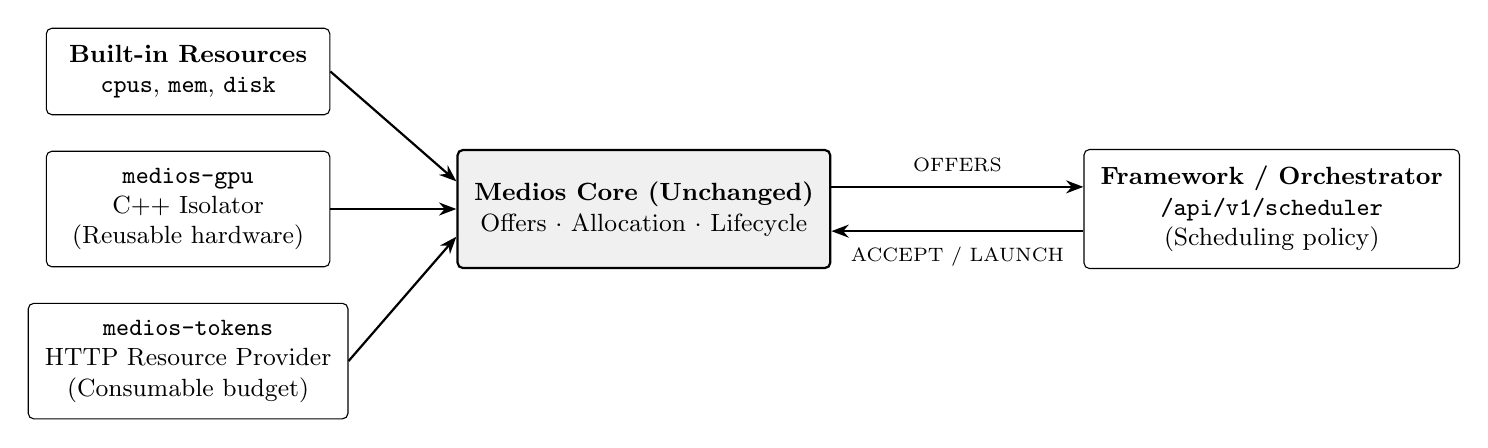
\begin{tikzpicture}[
  box/.style={rectangle, draw, rounded corners=2pt, align=center, inner sep=6pt, minimum width=3.6cm, font=\small},
  core/.style={box, fill=black!6, thick, minimum width=4.0cm, minimum height=1.5cm},
  arr/.style={-{Stealth[length=2.2mm]}, thick}
]
  \node[core] (core) {\textbf{Medios Core (Unchanged)}\\Offers $\cdot$ Allocation $\cdot$ Lifecycle};
  \node[box, left=1.6cm of core] (gpu) {\textbf{\texttt{medios-gpu}}\\C++ Isolator\\(Reusable hardware)};
  \node[box, above=0.45cm of gpu] (builtin) {\textbf{Built-in Resources}\\\texttt{cpus}, \texttt{mem}, \texttt{disk}};
  \node[box, below=0.45cm of gpu] (tok) {\textbf{\texttt{medios-tokens}}\\HTTP Resource Provider\\(Consumable budget)};
  \node[box, right=3.2cm of core, minimum height=1.5cm] (fw) {\textbf{Framework / Orchestrator}\\\texttt{/api/v1/scheduler}\\(Scheduling policy)};

  \draw[arr] (builtin.east) -- ([yshift=10pt]core.west);
  \draw[arr] (gpu.east) -- (core.west);
  \draw[arr] (tok.east) -- ([yshift=-10pt]core.west);
  \draw[arr] ([yshift=8pt]core.east) -- node[above=2pt, font=\scriptsize] {OFFERS} ([yshift=8pt]fw.west);
  \draw[arr] ([yshift=-8pt]fw.west) -- node[below=2pt, font=\scriptsize] {ACCEPT / LAUNCH} ([yshift=-8pt]core.east);
\end{tikzpicture}%
}
\caption{Compute scalars, hardware isolators, and external budget providers are co-offered through the same unmodified Medios broker.}
\label{fig:arch}
\end{figure}

\begin{table}[htbp]
\centering
\small
\begin{tabular}{@{}lll@{}}
\toprule
\textbf{Dimension} & \textbf{\texttt{medios-gpu}} & \textbf{\texttt{medios-tokens}} \\
\midrule
Resource & GPU capacity & API token budget \\
Source of truth & Host GPU hardware / driver & External API or local ledger \\
Resource behavior & Reusable & Consumable \\
Availability model & Device inventory \& allocation & Balance, reservations, refills \\
Lifecycle & Acquire $\rightarrow$ use $\rightarrow$ release & Reserve $\rightarrow$ spend $\rightarrow$ settle \\
Extension seam & C++ \texttt{Isolator} (\texttt{--modules}) & HTTP \texttt{ResourceProvider} \\
Restart safety & Sandbox device UUID checkpoint & Atomic JSON ledger checkpoint \\
Core modifications & None & None \\
\bottomrule
\end{tabular}
\caption{Comparison of \texttt{medios-gpu} (reusable hardware) and \texttt{medios-tokens} (consumable budget).}
\label{tab:pair}
\end{table}

\texttt{medios-tokens} subscribes to \texttt{medios-node} over \texttt{POST /api/v1/resource\_provider}, advertises its current balance via \texttt{UPDATE\_STATE}, authorizes launches on \texttt{PUBLISH\_RESOURCES}, and debits each accepted \texttt{task\_id} once on controller \texttt{TASK\_ADDED} events. An atomic local JSON checkpoint records \texttt{provider\_id}, remaining balance, and per-task entries across provider restarts.

\section{Task-Level Settlement Protocols}
\label{sec:settle}

At launch, a task reserves its worst-case spend. Because actual LLM spend is often below the reservation, settlement reconciles actual usage and returns unused credit (\texttt{reserved} $-$ \texttt{actual}) to the ledger. We implement two task-level settlement patterns.

\subsection{Pattern 1: Executor Finish Hook Settlement}
Medios runs an optional bounded post-exit command (\texttt{TaskInfo.finish}) inside the task's sandbox after the work command exits, regardless of exit code or framework kill. Under Pattern~1:
\begin{enumerate}
  \item The task writes its measured spend (for example, from OpenRouter's \texttt{/api/v1/generation?id=...} endpoint or token counts) to \texttt{./usage.json}.
  \item The finish hook reads the executor-injected \texttt{MEDIOS\_TASK\_ID} and \texttt{./usage.json}, then posts \texttt{\{"task\_id", "actual"\}} to \texttt{POST /settle}.
  \item If \texttt{./usage.json} is missing or malformed, the hook skips settlement and fails closed, keeping the full reservation debited.
\end{enumerate}

\subsection{Pattern 2: Per-Task Scoped Provider Keys}
Pattern~1 relies on cooperative reporting and cannot stop a runaway loop from overspending a shared API key. Pattern~2 enforces per-task ceilings at the upstream API via a \texttt{Provisioner} interface and an OpenRouter Management API adapter:
\begin{enumerate}
  \item Before launching \texttt{task\_id}, the framework calls \texttt{POST /provision} with \texttt{\{"task\_id", "limit"\}}.
  \item \texttt{medios-tokens} calls \texttt{POST /api/v1/keys} on OpenRouter, returns the secret key once to the caller for task environment injection, and persists only the opaque \texttt{key\_hash} in the ledger checkpoint. Raw secrets are not written to disk.
  \item When the controller emits a terminal \texttt{TASK\_UPDATED} event (\texttt{TASK\_FINISHED}, \texttt{TASK\_FAILED}, \texttt{TASK\_KILLED}, \texttt{TASK\_LOST}, etc.), \texttt{medios-tokens} reads settled usage (\texttt{GET /api/v1/keys/\{hash\}}), revokes the key (\texttt{DELETE /api/v1/keys/\{hash\}}), settles the ledger, and emits \texttt{UPDATE\_STATE}.
\end{enumerate}

\subsection{Exclusion of Account-Level Treasury Polling}
Periodic polling of an upstream provider's account-level credit balance is excluded. Upstream billing lag (seconds to minutes) causes an account poller to re-advertise credit already committed to in-flight tasks, breaking the hard spend cap. Task-scoped settlement avoids double-advertising.

\section{Experimental Evaluation}
\label{sec:eval}

Our evaluation asks three questions against unmodified \texttt{medios-controller}, \texttt{medios-node}, and \texttt{medios-executor} binaries running alongside \texttt{medios-tokens} on macOS (Apple Silicon):

\begin{enumerate}
  \item \textbf{Accounting safety:} Does finish-hook settlement recover unused budget on both clean exits and task failures while failing closed when a task crashes without reporting usage?
  \item \textbf{Upstream enforcement:} Can the provider enforce hard spend caps at an external LLM API and automatically revoke credentials on task termination without persisting raw secrets?
  \item \textbf{Multi-agent contention:} Does exposing live remaining budget inside cluster offers let a scheduling policy eliminate stranded workflows that occur under naive contention, without changing the broker or provider?
\end{enumerate}

\subsection{Finish-Hook Settlement Under Success, Failure, and Crash}
In a consumable budget ledger, two failure modes pull in opposite directions: refusing to settle failed tasks leaks capacity unnecessarily, whereas refunding a task that crashed without reporting usage can over-credit the pool. To test both boundaries, we initialized a local cluster with \texttt{token\_budget=100} and ran three sequential tasks via \path{examples/finish-hook-settle/smoke.py}, each reserving $25$ units:

\begin{itemize}
  \item The first task exited cleanly after recording $18$ units of spend. The finish hook settled the task and returned $7$ unused units, bringing the next offer to $82$.
  \item The second task exited with status~1 after recording $10$ units of partial spend. Because Medios runs finish hooks regardless of work exit status, the hook still settled the task and returned $15$ unused units, bringing the next offer to $72$.
  \item The third task crashed without writing \texttt{./usage.json}. The hook refused to guess, issued no refund, and left the full $25$-unit reservation debited, bringing the next offer to $47$.
\end{itemize}

This confirms that cooperative settlement can reclaim unused reservations across normal and failing runs without compromising fail-closed accounting on unverified crashes.

\subsection{Live OpenRouter Scoped-Key Enforcement}
Cooperative hooks cannot stop a runaway loop from overspending a shared API key. To verify hard upstream enforcement end-to-end, we configured \texttt{medios-tokens} with an OpenRouter Management API key loaded from Google Secret Manager into \texttt{OPENROUTER\_PROVISIONING\_KEY} and ran a live task against \texttt{https://openrouter.ai}.

Before launch, \texttt{POST /provision} minted a $\$0.05$-capped key (\texttt{hash\_prefix=8d6fe40e513d}). Inspecting the ledger checkpoint file on disk confirmed that only \texttt{key\_hash} was written; the raw secret never appeared on disk. A live \texttt{openai/gpt-4o-mini} completion succeeded using the minted key. When the controller emitted \texttt{TASK\_FINISHED}, \texttt{medios-tokens} automatically read key usage, revoked the key via \texttt{DELETE /api/v1/keys/\{hash\}}, and published updated capacity via \texttt{UPDATE\_STATE} ($1.00 \rightarrow 0.95 \rightarrow 1.00$). A follow-up query to \texttt{GET /api/v1/keys} confirmed zero \texttt{medios-*} keys remained in the account.

One practical limitation surfaced during this test: for a sub-second completion costing a few millionths of a dollar, OpenRouter's per-key usage counter and edge deletion cache lagged by roughly $2\text{--}3$\,s. Multi-second agent runs settle accurately, while sub-second calls motivate an optional pre-settle delay.

\subsection{Multi-Agent Contention vs.\ Budget-Aware Orchestration}
A hard budget cap prevents overspending, but it does not guarantee useful work when multiple agents compete for the same pool. To isolate the effect of scheduling policy over an unchanged broker, we constructed a six-workflow workload (\path{examples/multi-agent-budget/benchmark.py}) sharing a $100$-unit \texttt{token\_budget}:

\begin{itemize}
  \item \textbf{Four high-value research chains,} each consisting of three sequential steps (\texttt{plan}: $5$, \texttt{gather}: $8$, \texttt{synthesize}: $7$; $20$ units per chain, $80$ total). A chain produces value only if all three steps complete.
  \item \textbf{Two low-value background digests,} each requiring a single step costing $18$ units on a standard model, or $6$ units if routed to a cheaper model tier.
\end{itemize}

The $100$-unit pool is deliberately sized so that all six workflows can complete ($80 + 12 = 92$ units) if the scheduler coordinates spend, yet cannot complete if tasks grab blanket worst-case reservations in arrival order. We ran this workload on two fresh clusters using identical \texttt{medios-controller}, \texttt{medios-node}, and \texttt{medios-tokens} binaries, varying only the scheduler:

\begin{itemize}
  \item \textbf{Case 1 (Naive FIFO Queue):} Tasks pull from an interleaved FIFO queue and reserve a conservative $25$ units per step, with no chain admission or model routing. Because the two background digests run early on the standard model ($36$ units) and the remaining budget is split across steps~1 and~2 of the four research chains ($44$ units), only $20$ units remain when step~3 arrives. That remainder sits below the $25$-unit reservation threshold, so every offer is declined and all four research chains are stranded at step~2 of~3. \texttt{medios-tokens} holds the $100$-unit ceiling, but $44$ units are wasted on incomplete work.
  \item \textbf{Case 2 (Smart Budget Orchestrator):} The orchestrator reads live \texttt{token\_budget} directly from incoming \texttt{OFFERS} and applies three policies: (a)~full-chain admission, starting a research chain only when remaining budget covers its $20$-unit total; (b)~tighter per-step reservations ($8, 10, 9$) with immediate settlement recycling; and (c)~watermark routing, downgrading background digests to the $6$-unit model tier once remaining budget falls to $25$ or below. All four research chains finish first ($80$ units), after which both digests run on the cheaper tier ($12$ units), completing all six workflows with $8$ units to spare.
\end{itemize}

\begin{table}[t]
\centering
\small
\begin{tabular}{@{}lcc@{}}
\toprule
\textbf{Metric} & \textbf{Case 1: Naive FIFO Queue} & \textbf{Case 2: Smart Orchestrator} \\
\midrule
Starting \texttt{token\_budget} & $100.0$ & $100.0$ \\
High-value workflows (3-step) & $0 / 4$ & $\mathbf{4 / 4}$ \\
Low-value background digests & $2 / 2$ & $\mathbf{2 / 2}$ \\
Total workflows completed & $2 / 6$ & $\mathbf{6 / 6}$ \\
Budget wasted on stranded work & $44.0$ & $\mathbf{0.0}$ \\
Remaining \texttt{token\_budget} & $20.0$ (fragmented $< 25$) & $8.0$ \\
Wall-clock time (live cluster) & $8.89$\,s & $\mathbf{8.35}$\,s \\
Changes to broker / provider & None & None \\
\bottomrule
\end{tabular}
\caption{Live multi-agent benchmark on two fresh Medios clusters with \texttt{medios-tokens}.}
\label{tab:bench}
\end{table}

Table~\ref{tab:bench} summarizes the measured outcomes. The improvement comes entirely from giving the scheduler visibility into remaining budget at offer time; neither Medios core nor \texttt{medios-tokens} changed between runs.

\section{Related Work}
\label{sec:related}

Prior systems address LLM token budgets and agent resources at four layers outside the cluster offer loop:

\begin{itemize}
  \item \textbf{L7 AI gateways:} LiteLLM, Portkey, and Envoy AI Gateway enforce virtual keys and token-bucket limits on HTTP traffic, returning HTTP~429 once a cap is reached. Because the cluster scheduler does not see gateway balances, tasks still claim compute and execute partial chains before failing.
  \item \textbf{Algorithmic budget planners:} BAMAS~\cite{yang2025bamas}, ZEBRA~\cite{hamri2026zebra}, and BudgetThinker~\cite{budgetthinker2025} allocate budgets across agent topologies, pipeline phases, or reasoning tokens. These policies can run as frameworks consuming Medios offers.
  \item \textbf{Language-level enforcement:} A recent empirical study of 63 LLM-agent budget overruns~\cite{tokenbudgets2026} uses affine Rust types to prevent single-process retry loops from bypassing caps. \texttt{medios-tokens} operates at the cluster boundary across languages and containers.
  \item \textbf{Agent OS and cluster managers:} AIOS~\cite{mei2024aios}, AgentCgroup~\cite{agentcgroup2025}, Kubernetes Extended Resources, Ray custom resources, and Slurm GRES/TRES manage reusable slots or post-hoc accounting rather than real-time consumable ledgers with task-scoped settlement.
\end{itemize}

\section{Limitations and Future Work}
\label{sec:limits}

\subsection{Current Limitations}
Four practical limitations bound this research preview:

\begin{itemize}
  \item \textbf{Single-node locality:} In Medios today, every \texttt{Offer} is bound to a single \texttt{node\_id}, and \texttt{/api/v1/resource\_provider} exists only on \texttt{medios-node}. While a single provider suffices for dense single-host multi-agent experiments (where dozens of lightweight containers share one machine and one experiment budget), scaling the same pool across multiple nodes hits a locality boundary: running independent providers fragments the budget across nodes, whereas advertising one global balance from every node risks double-spending concurrent accepts.
  \item \textbf{Reservation--utilization tradeoff:} Tasks must reserve an upper bound at offer-accept time before actual LLM spend is known. Conservative reservations temporarily lock capital until settlement completes, whereas overly tight reservations risk terminating long-running agents before their final step.
  \item \textbf{Upstream billing lag:} As observed in Experiment~2, external provider usage counters and key-revocation edge caches are eventually consistent ($2\text{--}3$\,s on OpenRouter, and longer on batch or metered APIs). Settling immediately on task completion can under-report micro-spend, while waiting delays credit recycling.
  \item \textbf{No mid-flight budget renegotiation:} Once a task launches with a hard-capped key, it cannot request an incremental top-up through the broker if an intermediate step consumes more tokens than expected.
\end{itemize}

\subsection{Future Research Directions}
\begin{itemize}
  \item \textbf{Multi-node global budgets (two architectural paths):} Supporting a cluster-wide token pool does not require a separate secondary broker. Without modifying Medios core, a single centralized \texttt{medios-tokens} process can hold one global ledger, subscribe to all $N$ nodes over \texttt{/api/v1/resource\_provider}, and dynamically partition and rebalance per-node budget slices via \texttt{UPDATE\_STATE} as tasks debit and settle. To support an \emph{unpartitioned} global sum where any node can draw from the full pool, Medios core can complete controller-level External Resource Providers: the host-agnostic \texttt{ResourceProviderManager}, registrar, and \texttt{resource\_provider\_registry} proto scaffolding already exist in the codebase, leaving controller-side HTTP wiring and global-resource allocation (with cross-node offer rescission on accept) as the core open broker problem.
  \item \textbf{Dynamic leased credential brokers:} Implementing the \texttt{Provisioner} interface against a leased-secret broker such as OpenBao would generalize task-scoped credentials, lease TTLs, and automatic terminal revocation beyond OpenRouter to arbitrary paid APIs, database quotas, or external tools.
  \item \textbf{Online reservation sizing and policy integration:} Coupling live \texttt{token\_budget} offers with schedulers that learn per-step spend distributions online---or run algorithmic allocators such as ZEBRA~\cite{hamri2026zebra} and BAMAS~\cite{yang2025bamas}---could tighten reservations automatically without stranding multi-step workflows.
  \item \textbf{Broader non-hardware resource classes:} Testing the same HTTP \texttt{ResourceProvider} seam on sliding-window rate limits (TPM/RPM), exclusive physical lab equipment, or human-in-the-loop review capacity will clarify where the offer abstraction holds and where broker changes become necessary.
\end{itemize}

\section{Reproducibility}
Source code, unit tests (\texttt{go test -race ./...}), the finish-hook smoke harness (\path{examples/finish-hook-settle/smoke.py}), and the multi-agent benchmark (\path{examples/multi-agent-budget/benchmark.py}) are available at \url{https://github.com/medios-lab/medios-tokens} under the Apache~2.0 license.

{\small
\bibliographystyle{plain}
\bibliography{refs}
}

\end{document}
